\subsection{Fichier de tests}
	Le programme est exécuté avec le fichier \texttt{tests/test\_complet}:
	\inputminted[frame=single,label=Test]{text}{../tests/test_complet}
	On obtient alors le résultat suivant: 
	\begin{multicols}{2}
	\inputminted[breaklines=true,frame=single,label=Resultat]{text}{../tests/resultat_test_complet}
	\end{multicols}

	Pour ce fichier de tests, nous avons effectué un suivi avec l'outil \texttt{ddd}.
	\begin{figure}[H]
		\centering 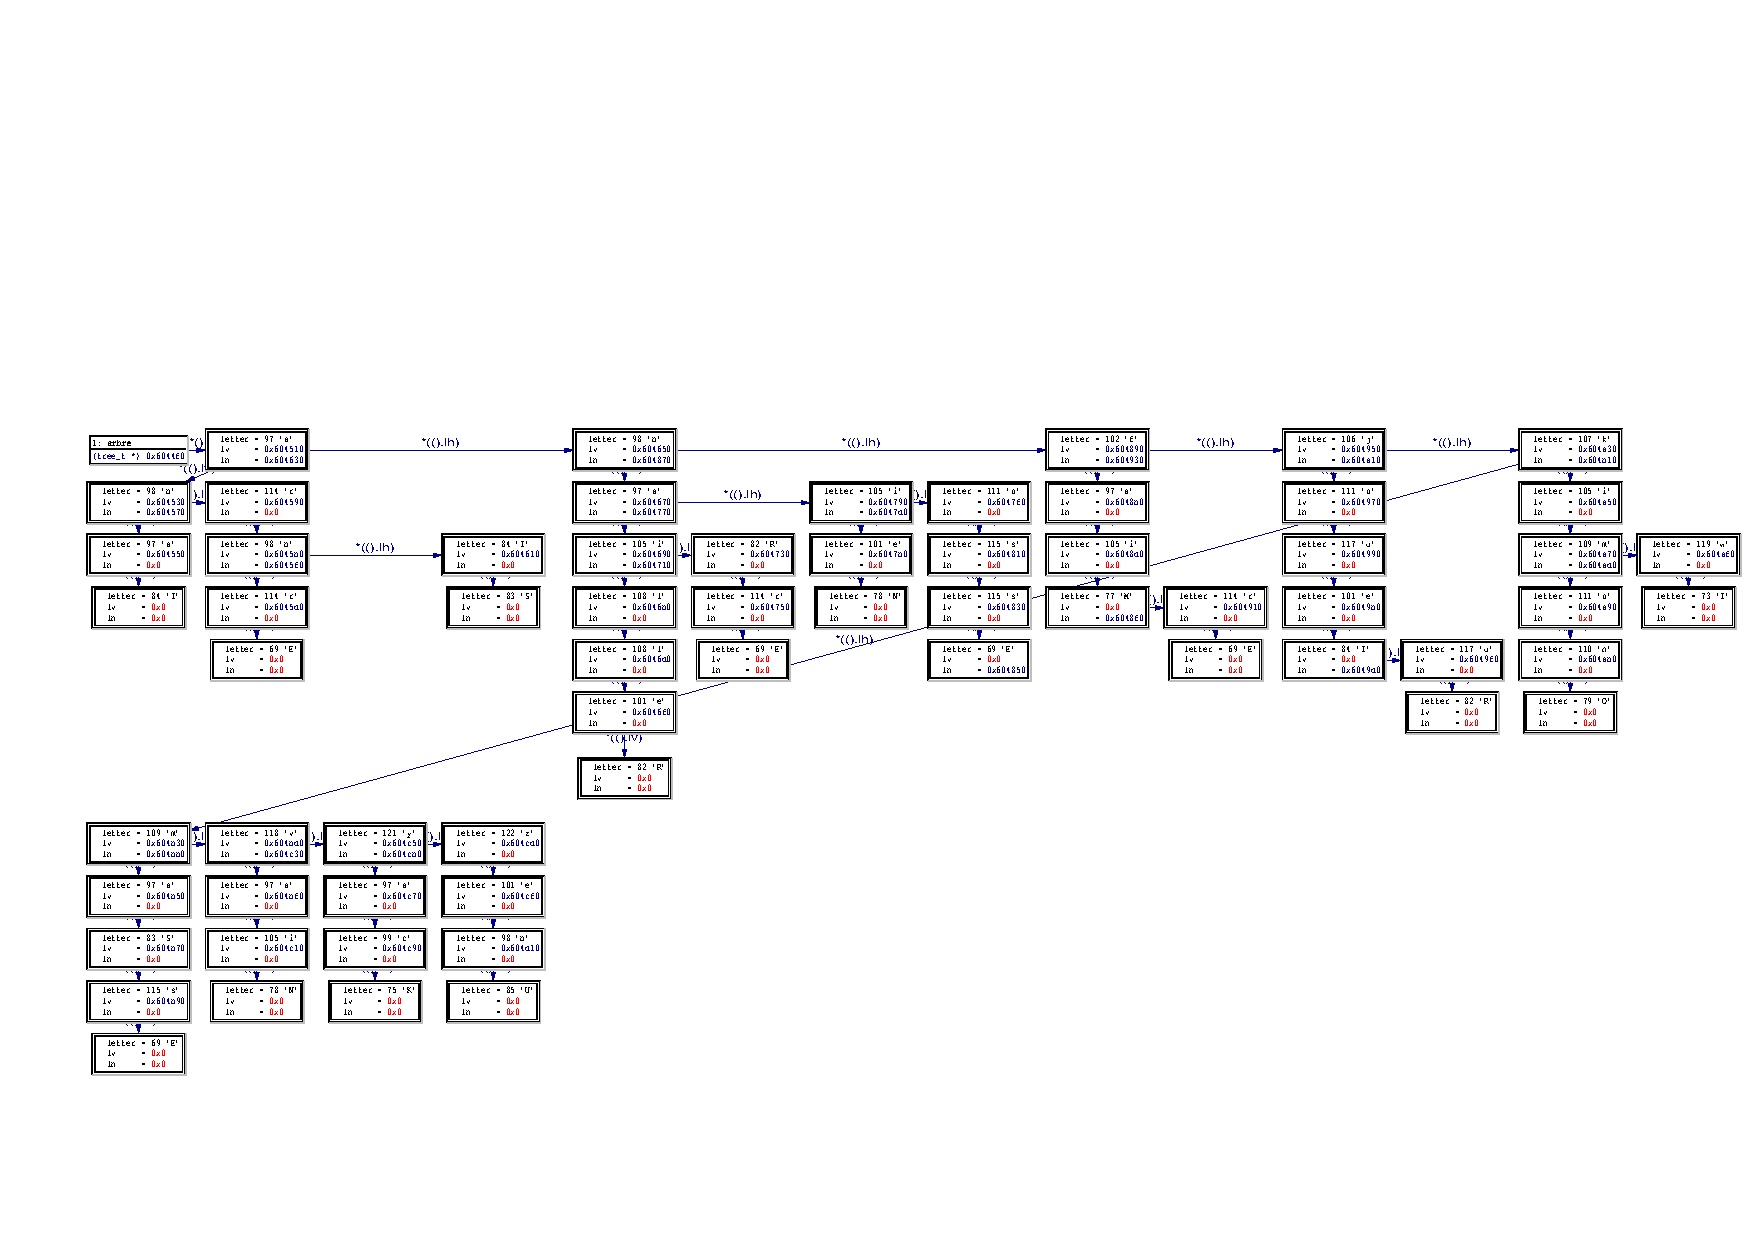
\includegraphics[angle=90,scale=0.82,trim=1cm 0cm 0cm 5cm,clip=true]{../tests/ddd_creation}
		\caption{Création de l'arbre}
	\end{figure}
	\begin{figure}[H]
		\centering 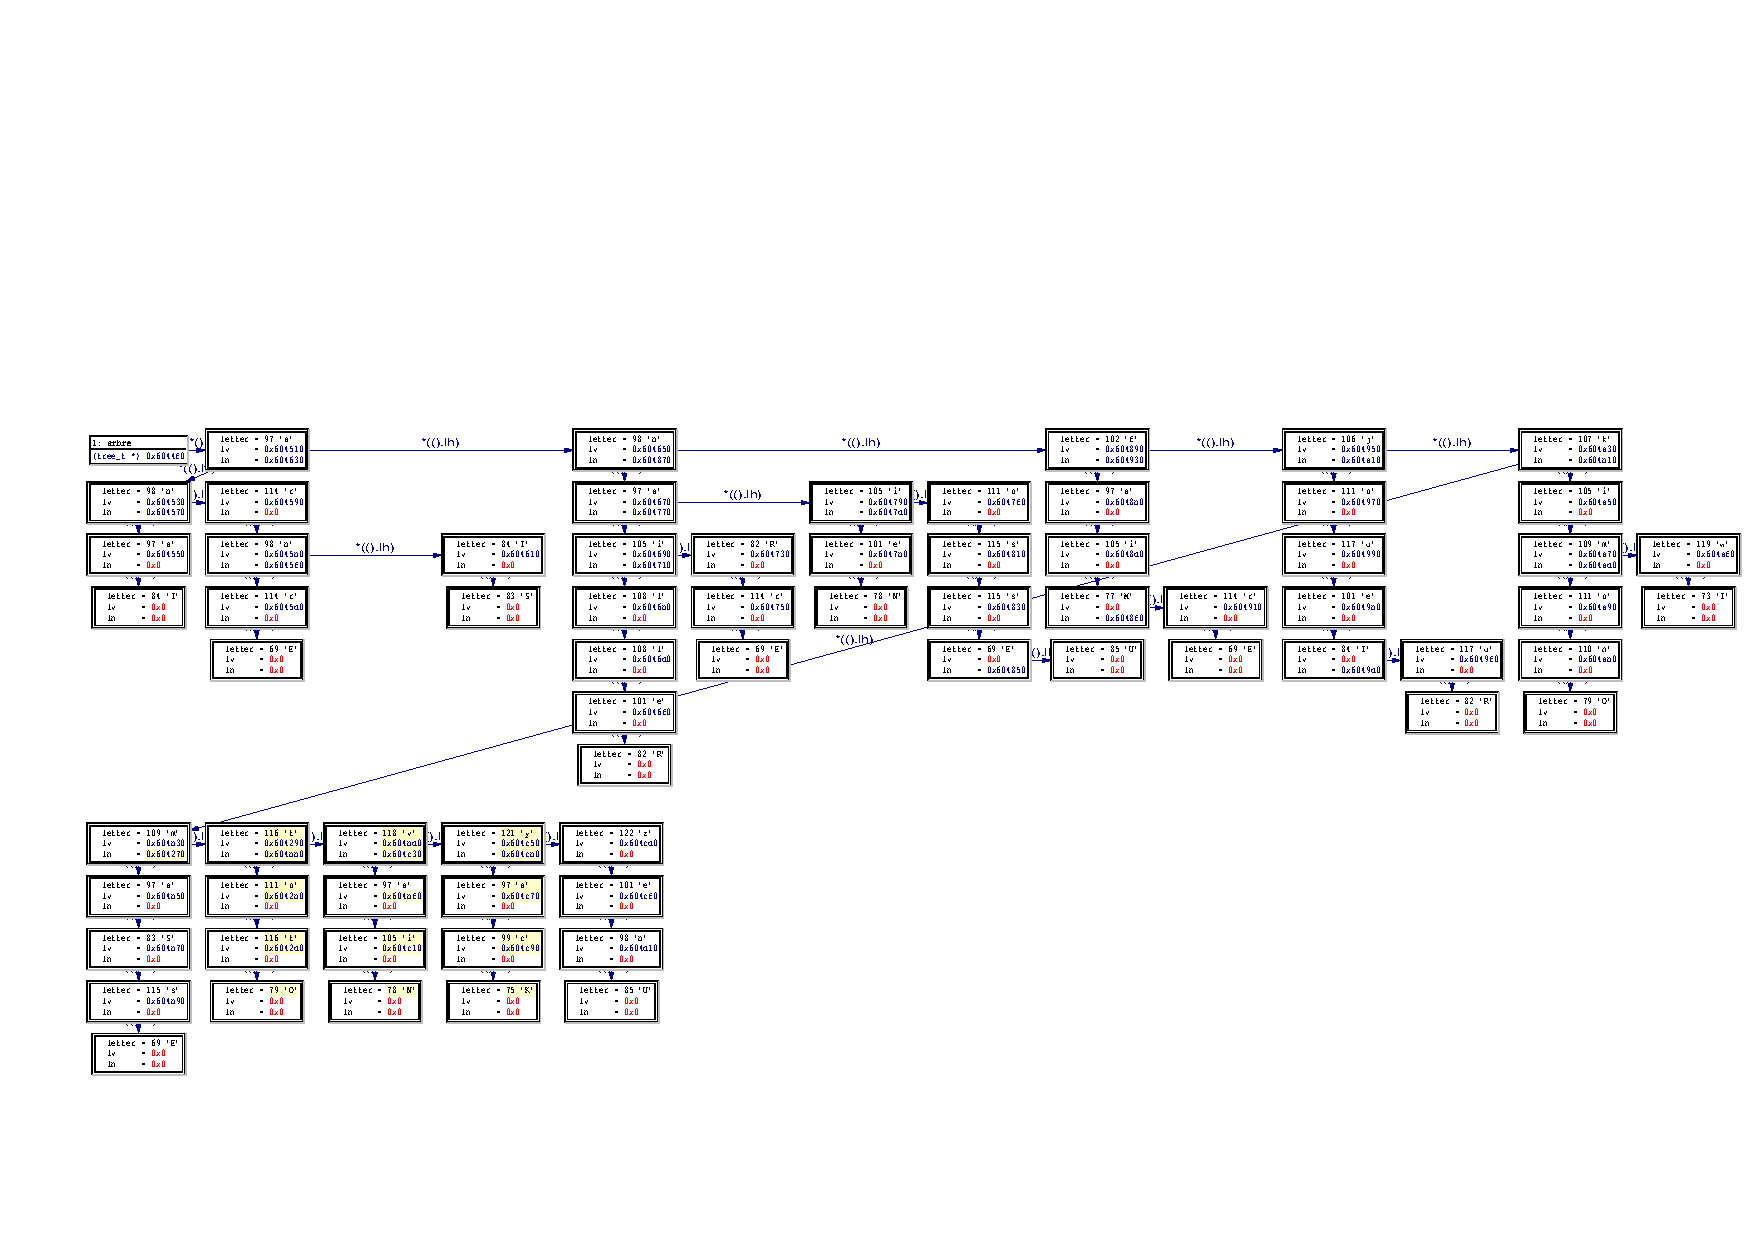
\includegraphics[angle=90,scale=0.82,trim=1cm 0cm 0cm 5cm,clip=true]{../tests/ddd_insertion_toto}
		\caption{Insertion de "toto"}
	\end{figure}
	\begin{figure}[H]
		\centering 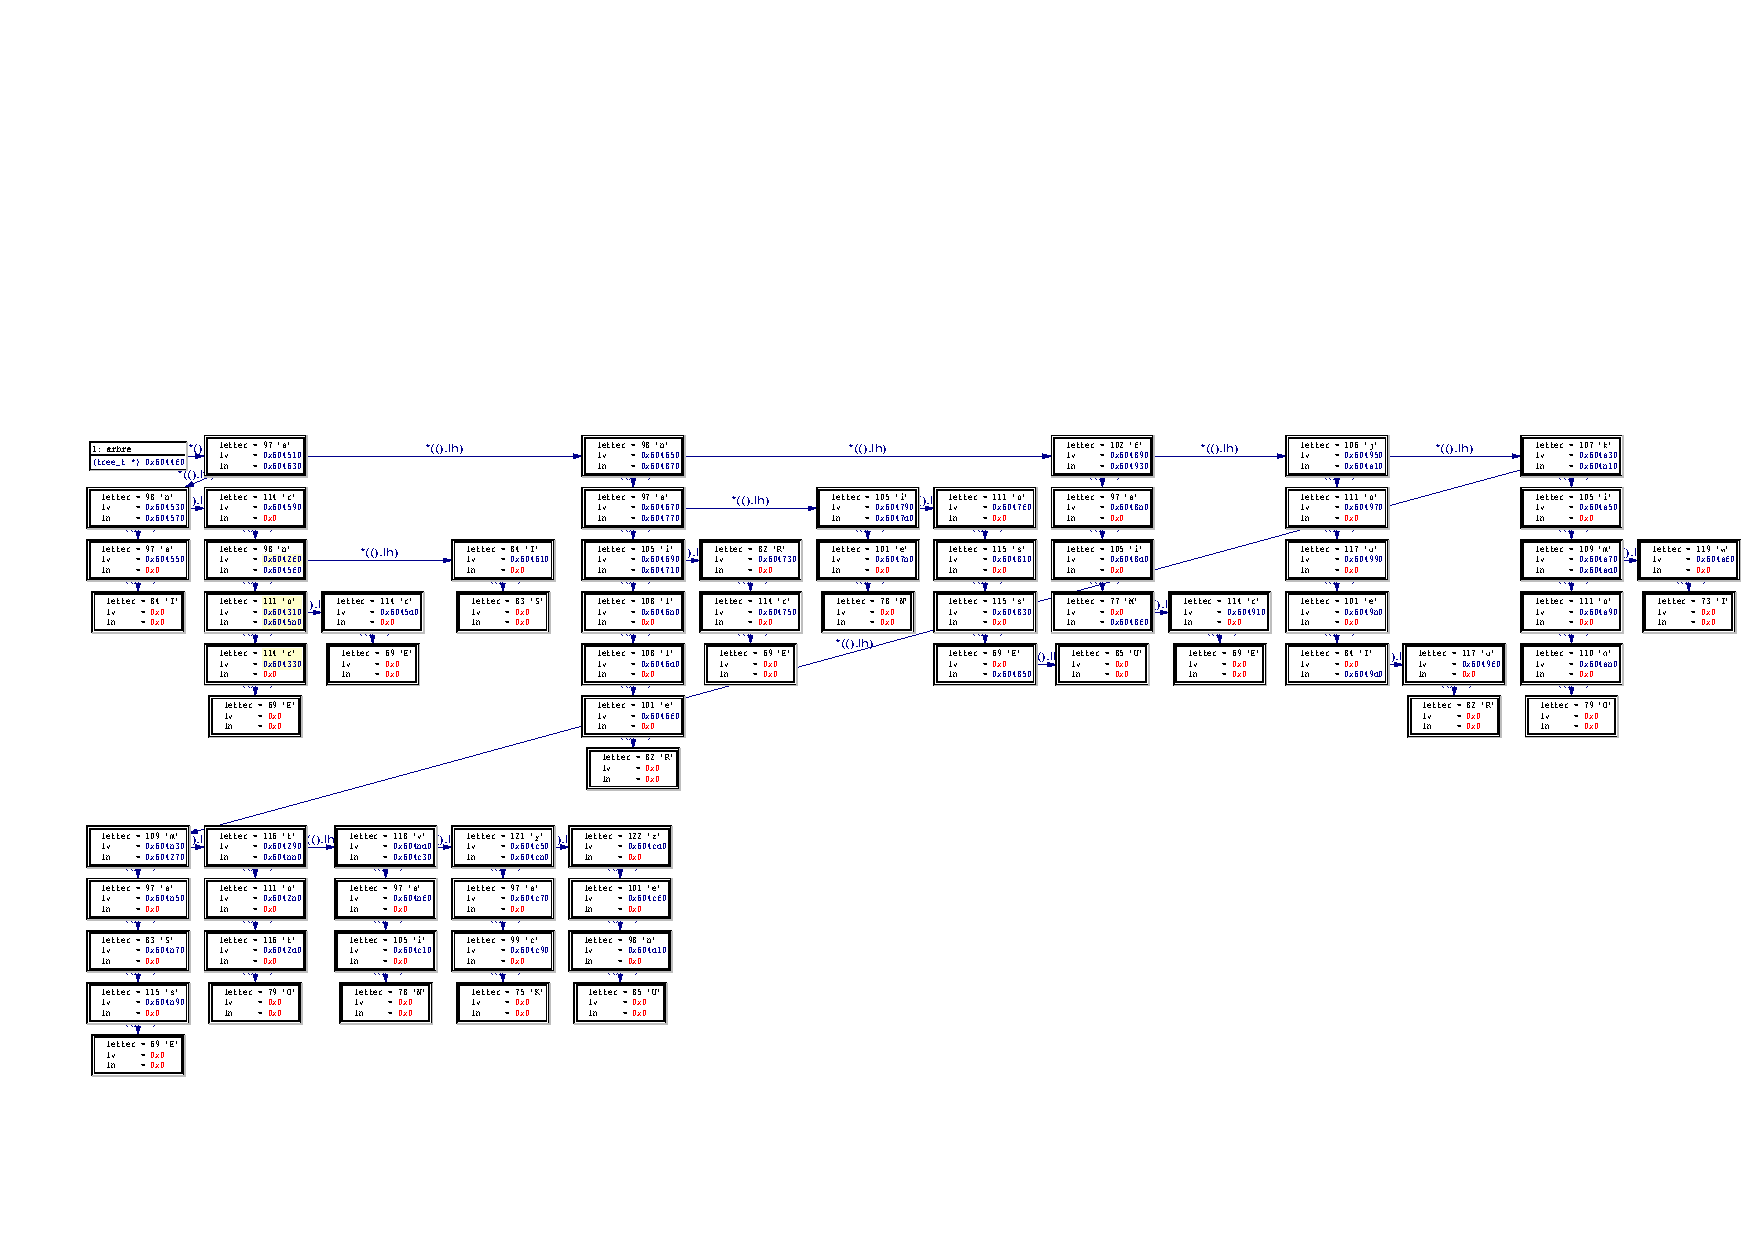
\includegraphics[angle=90,scale=0.82,trim=1cm 0cm 0cm 5cm,clip=true]{../tests/ddd_insertion_arbore}
		\caption{Insertion de "arbore"}
	\end{figure}
	\begin{figure}[H]
		\centering 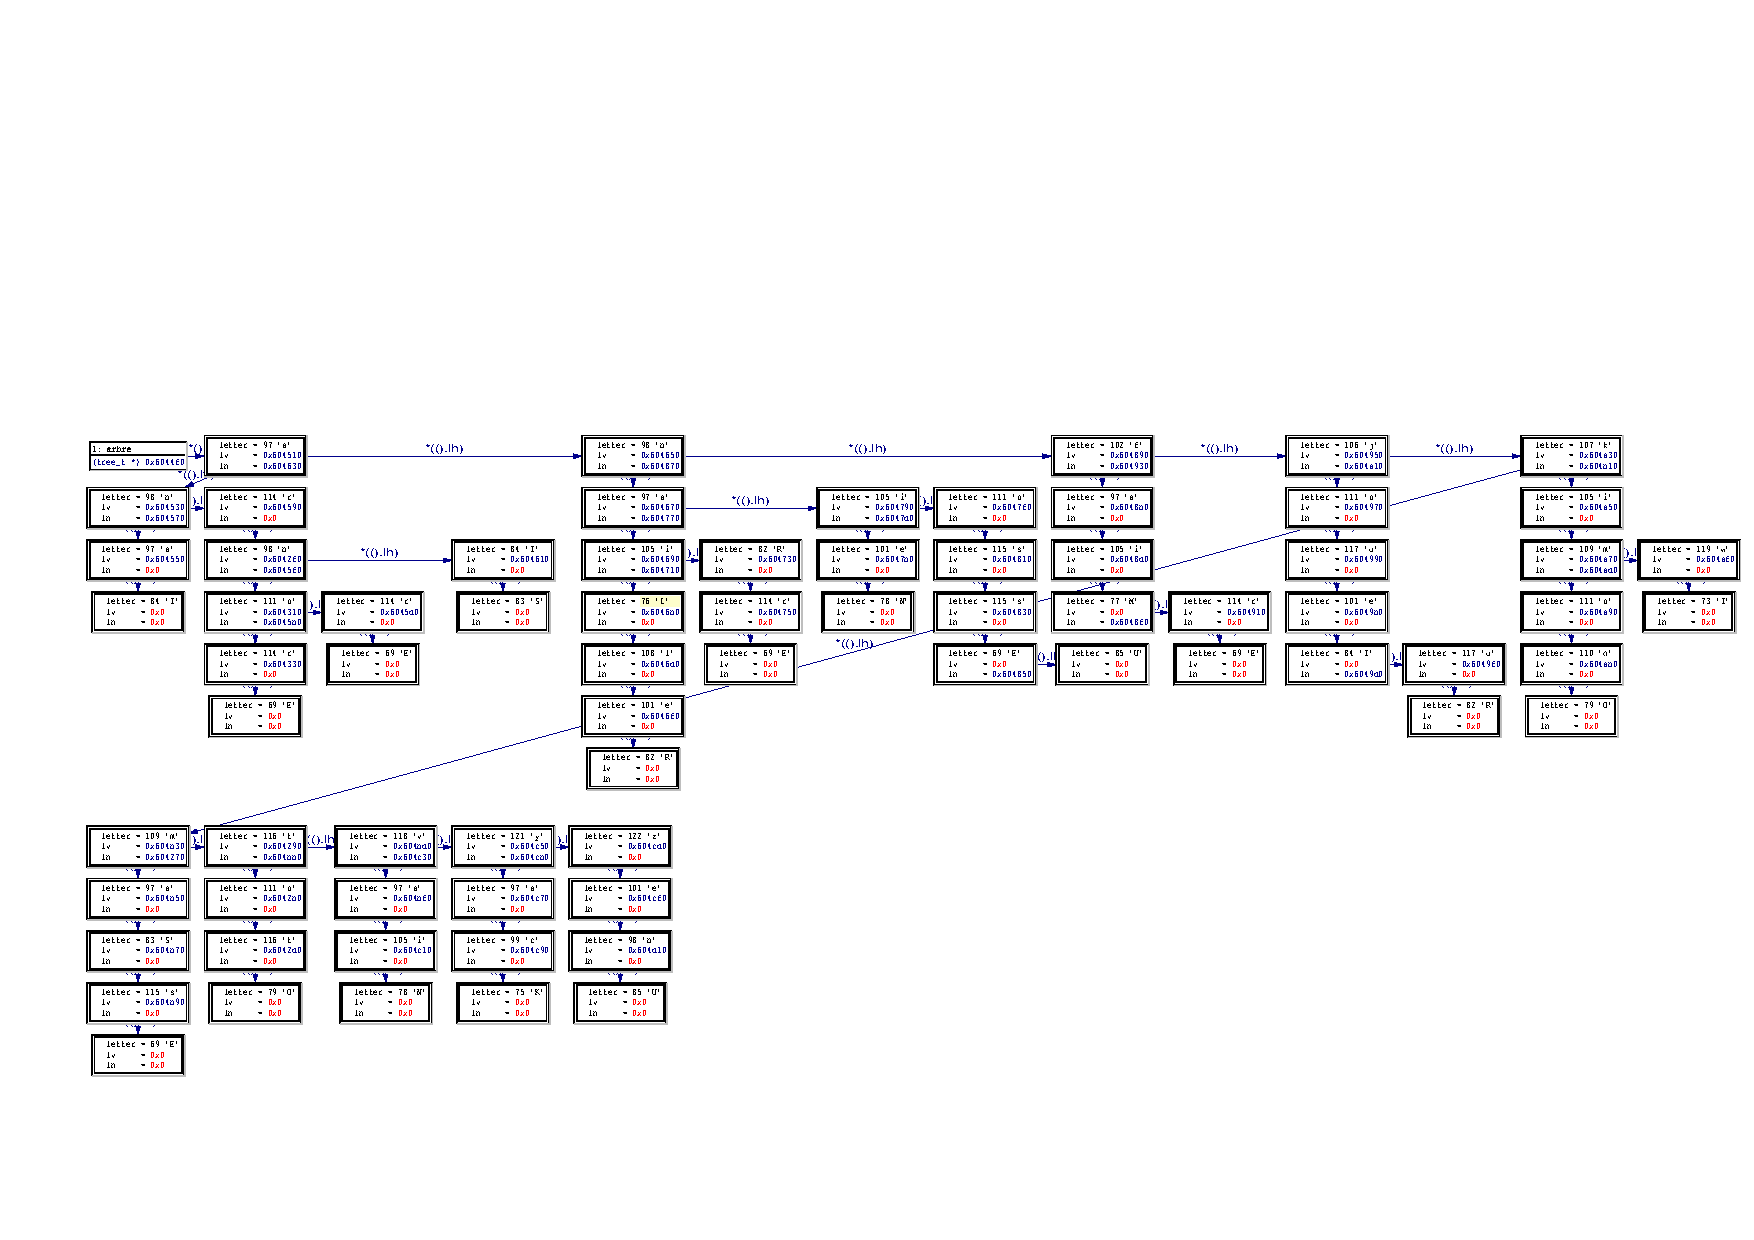
\includegraphics[angle=90,scale=0.82,trim=1cm 0cm 0cm 5cm,clip=true]{../tests/ddd_insertion_bail}
		\caption{Insertion de "bail"}
	\end{figure}
	\begin{figure}[H]
		\centering 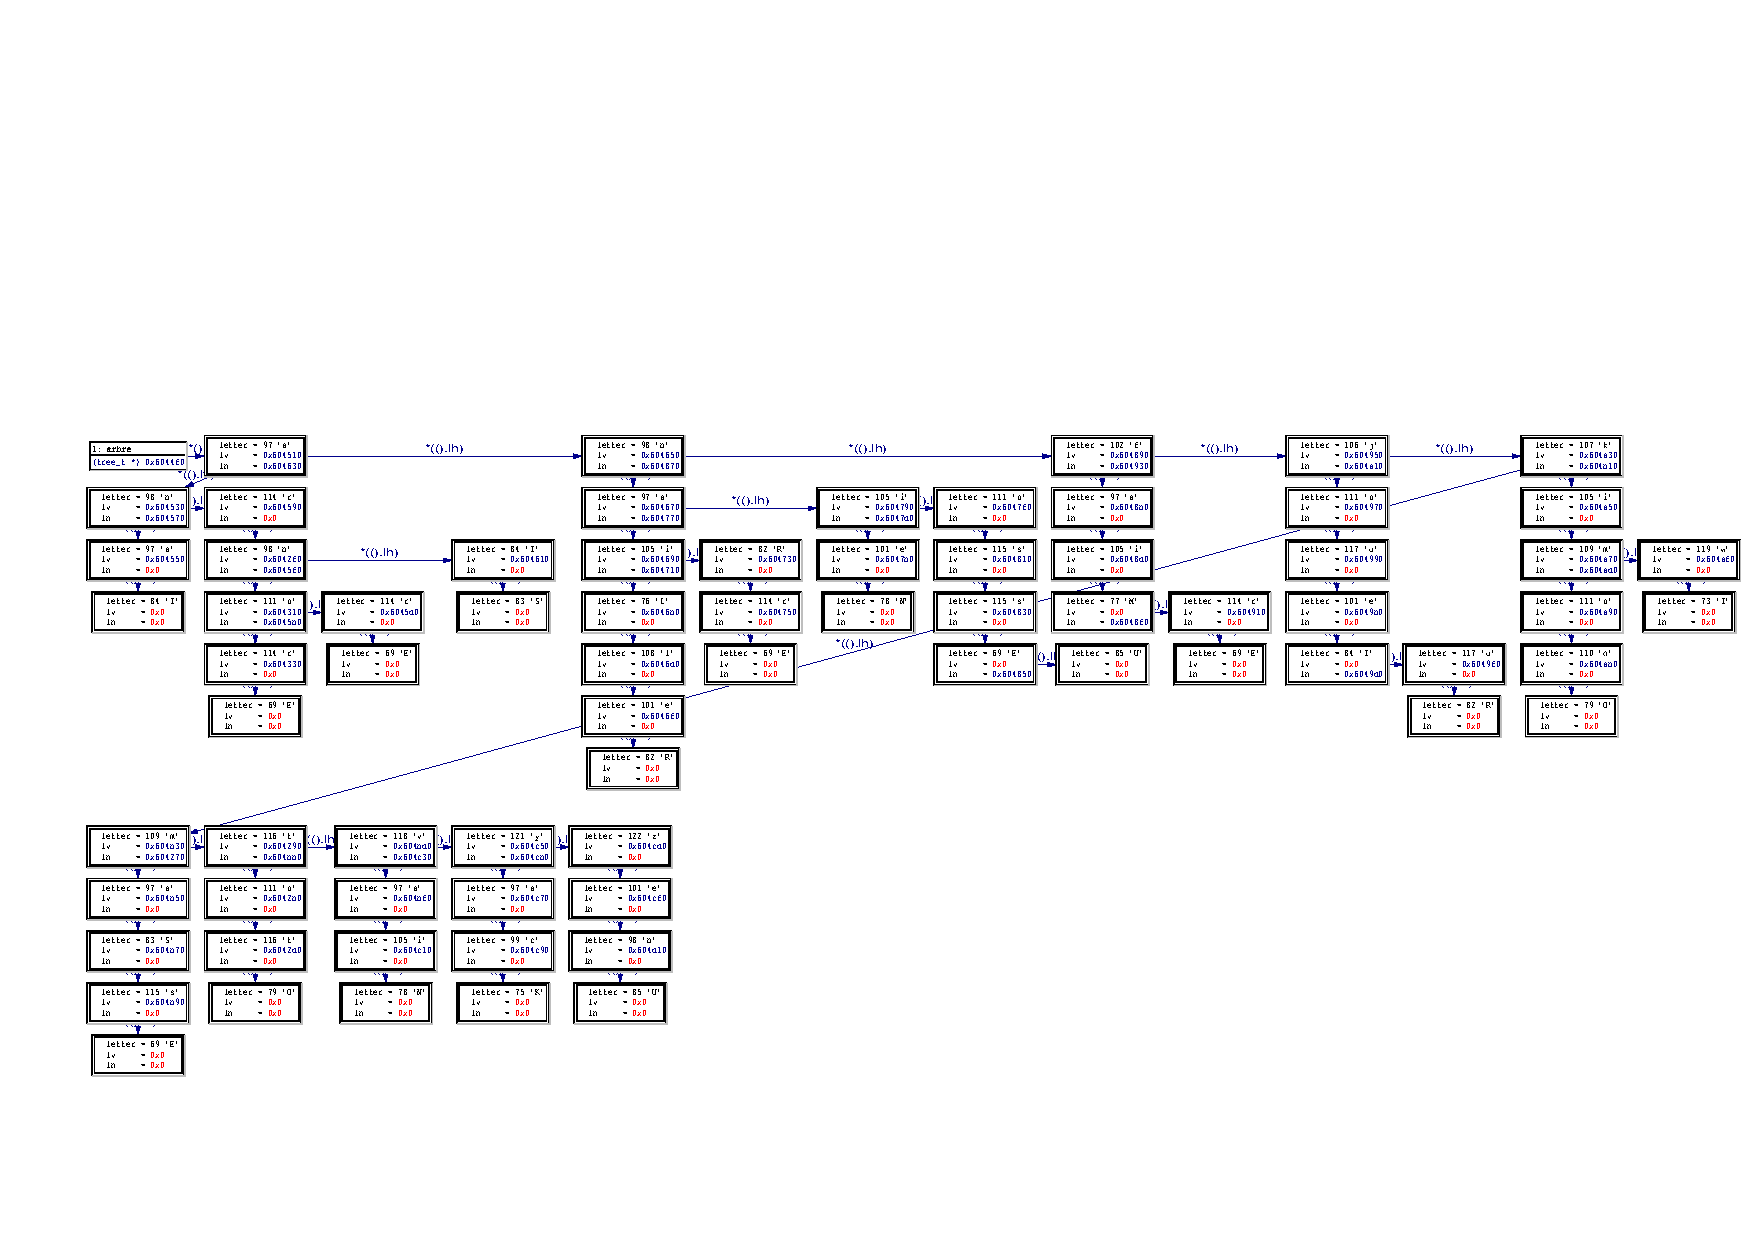
\includegraphics[angle=90,scale=0.82,trim=1cm 0cm 0cm 5cm,clip=true]{../tests/ddd_insertion_barre}
		\caption{Insertion de "barre"}
	\end{figure}
	\begin{figure}[H]
		\centering 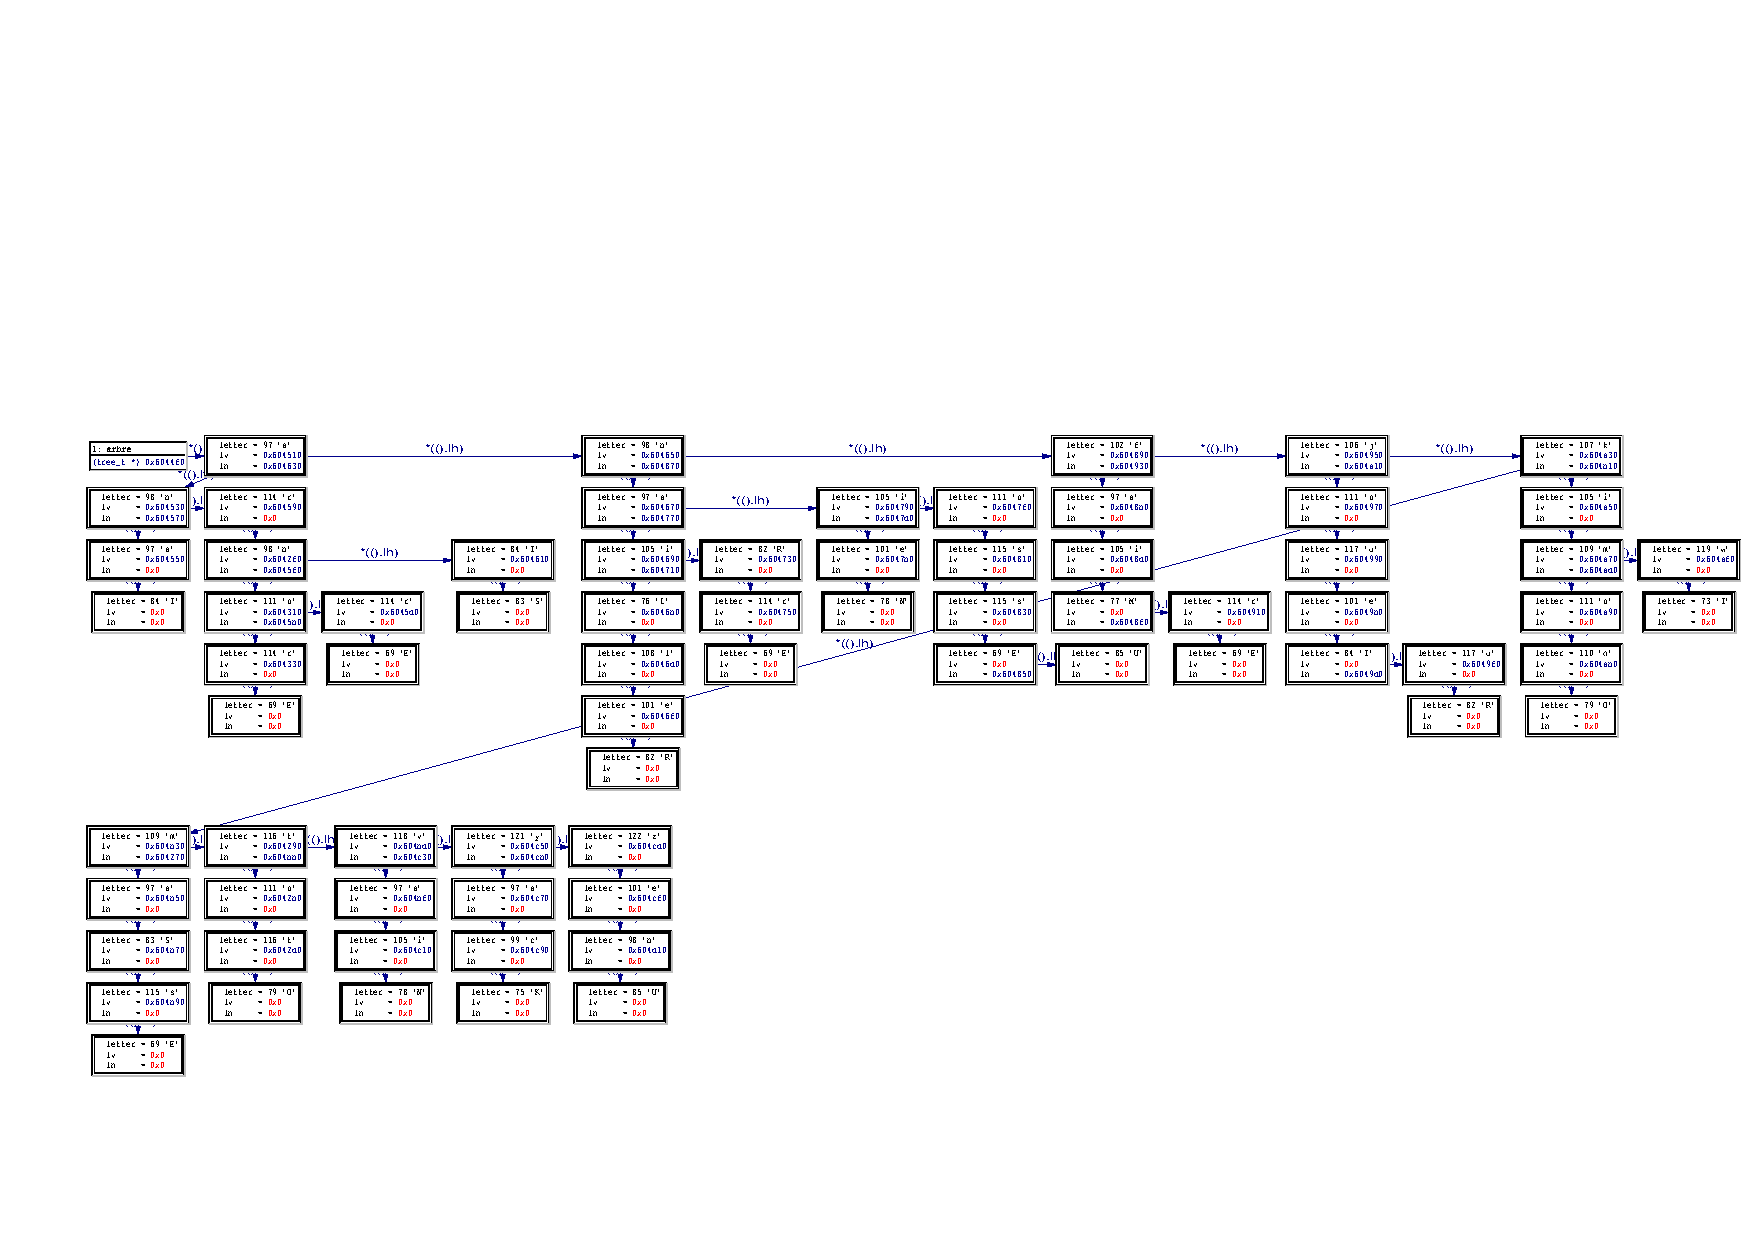
\includegraphics[angle=90,scale=0.82,trim=1cm 0cm 0cm 5cm,clip=true]{../tests/ddd_insertion_mot_vide}
		\caption{Insertion du mot vide}
	\end{figure}
	\begin{figure}[H]
		\centering 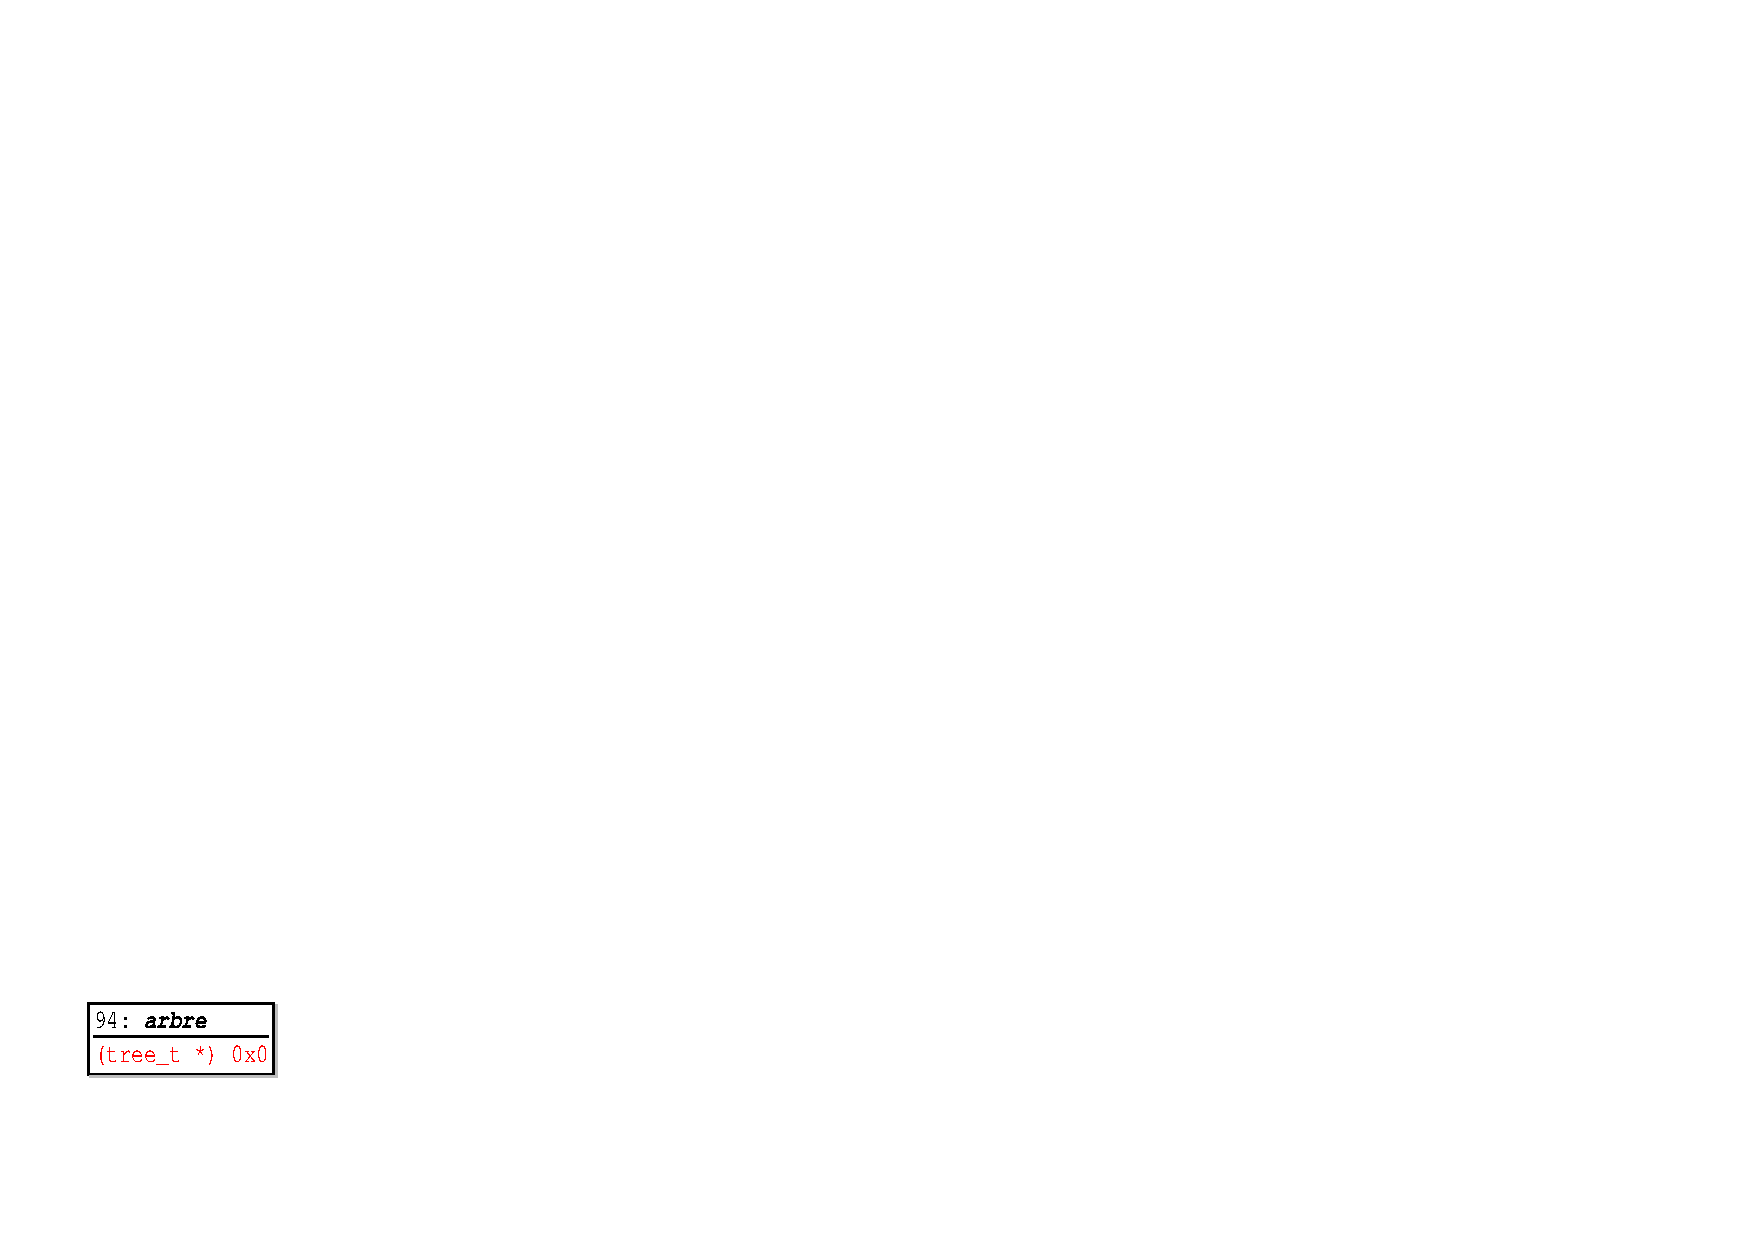
\includegraphics[scale=0.82,trim=1cm 2cm 24.5cm 16cm,clip=true]{../tests/ddd_suppression}
		\caption{Suppression de l'arbre}
	\end{figure}
	\begin{figure}[H]
		\centering 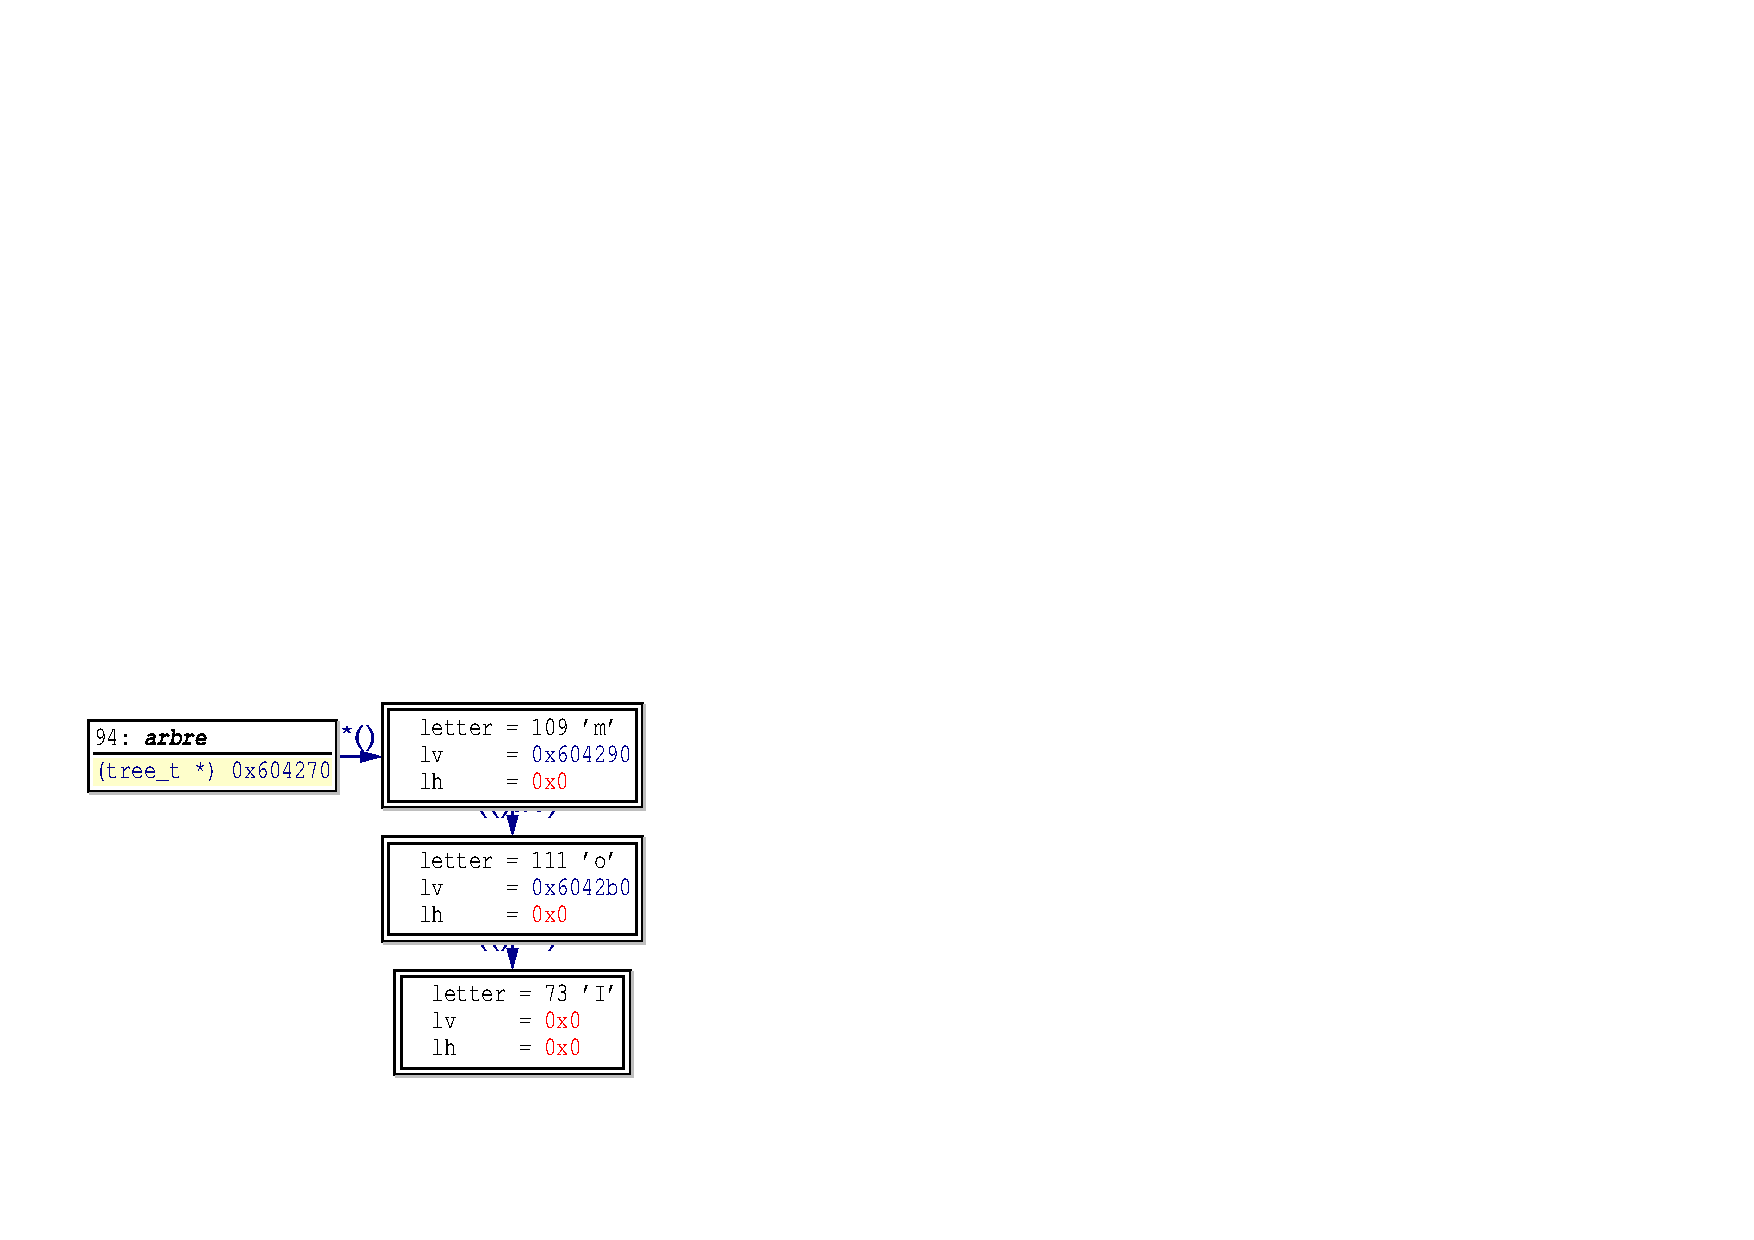
\includegraphics[scale=0.82,trim=1cm 2.5cm 18cm 11cm,clip=true]{../tests/ddd_insertion_moi}
		\caption{Insertion de "moi"}
	\end{figure}

	Le programme est exécuté avec le fichier \texttt{tests/test\_creation}:
	\inputminted[frame=single,label=Test]{text}{../tests/test_creation}
	\newpage
	On obtient alors le résultat suivant: 
	\inputminted[breaklines=true,frame=single,label=Resultat]{text}{../tests/resultat_test_creation}

	\newpage
	Le programme est exécuté avec le fichier \texttt{tests/test\_insertion}:
	\inputminted[frame=single,label=Test]{text}{../tests/test_insertion}
	On obtient alors le résultat suivant: 
	\begin{multicols}{2}
	\inputminted[breaklines=true,frame=single,label=Resultat]{text}{../tests/resultat_test_insertion}
	\end{multicols}

	\newpage
	Le programme est exécuté avec le fichier \texttt{tests/test\_motif}:
	\inputminted[frame=single,label=Test]{text}{../tests/test_motif}
	On obtient alors le résultat suivant: 
	\begin{multicols}{2}
	\inputminted[breaklines=true,frame=single,label=Resultat]{text}{../tests/resultat_test_motif}
	\end{multicols}

\subsection{Bonne utilisation de la mémoire}
	Pour vérifier la bonne libération de la mémoire, nous avons utilisé \texttt{valgrind} avec le programme seul et le fichier de test complet. Aucun bloc de mémoire n'est perdu, le retour texte de valgrind est présenté en figure \ref{fig:valgrind}.
	\begin{figure}[H]
	  \inputminted[frame=single,label=Resultat Valgrind]{text}{../tests/valgrind_test}
	  \caption{Passage dans l'outil \texttt{valgrind}}
	  \label{fig:valgrind}
	\end{figure}
